\documentclass{article}
\usepackage{eecstex}
\usepackage{pgfplots}
\usepackage{physics}

\renewcommand{\thesubsection}{\thesection.\arabic{subsection}}
\renewcommand{\thesubsubsection}{\thesubsection.\alph{subsubsection}}
\renewcommand{\labelenumi}{\arabic{enumi}.}
\newcommand{\F}{\mathcal{F}}

\title{EE 120 HW 05}
\author{Bryan Ngo}
\date{2021-02-23}

\begin{document}

\maketitle

\section{DTFT Practice}

\subsection{}

\begin{align}
    x[n] &= \qty(\frac{1}{2})^{-n} u[-n - 1] \\
    \implies X(e^{j \omega}) &= \sum_{k \in \Z} \qty(\frac{1}{2})^{-k} u[-k - 1] e^{j \omega k} \\
    &= \sum_{k \leqslant -1} 2^k e^{-j \omega k} = \sum_{k \leqslant -1} (2e^{-j \omega})^k \\
    &= \sum_{k \geqslant 1} \qty(\frac{1}{2} e^{j \omega})^k = \frac{1}{1 - \frac{1}{2}e^{j \omega}} - 1 \\
\end{align}

\subsection{}

\begin{align}
    x[n] &=
    \begin{cases}
        n & |n| \leqslant 3 \\
        0 & \text{elsewhere}
    \end{cases} \\
    \implies X(e^{j \omega}) &= \sum_{k \in \Z} x[k] e^{-j \omega k} = \sum_{k \in [-3, 3]} k e^{-j \omega k} \\
    &= -3e^{3j \omega} - 2 e^{2j \omega} - e^{j \omega} + e^{-j \omega} + 2e^{-2j \omega} + 3e^{-3j \omega} \\
    &= 2j \sin(\omega) + 4j \sin(2\omega) + 6j \sin(3\omega)
\end{align}

\subsection{}

\begin{align}
    X(j \omega) &= \sum_{k \in \Z} (-1)^k \delta\qty(\omega - \frac{\pi}{2} k) \, d\omega \\
    \implies x[n] &= \frac{1}{2\pi} \int_{-\frac{\pi}{4}}^{\frac{7\pi}{4}} e^{j \omega n} \sum_{k \in \Z} (-1)^k \delta\qty(\omega - \frac{\pi}{2} k) \, d\omega \\
    &= \frac{1}{2\pi} \int_{-\frac{\pi}{4}}^{\frac{7\pi}{4}} \qty(-\delta\qty(\omega - \frac{\pi}{2}) + \delta(\omega - \pi) - \delta\qty(\omega - \frac{3\pi}{2}) + \delta(\omega - 2\pi)) e^{j \omega n} \, d\omega \\
    &= \frac{1}{2\pi} (-e^{j \frac{\pi}{2} n} + e^{j \pi n} - e^{j \frac{3\pi}{2} n} + e^{j 2\pi n}) = \frac{1}{2\pi} \qty(1 + (-1)^n + 2j \sin\qty[\frac{\pi}{2} n])
\end{align}

\section{Half Sample Delay Filter}

\begin{equation}
    \mathcal{H}[n] = x[n - k]
\end{equation}

\subsection{}

\begin{equation}
    h[n] = \delta[n - k]
\end{equation}

\subsection{}

\begin{align}
    H(e^{j \omega}) = \sum_{n \in \Z} \delta[n - k] e^{-j \omega n} = e^{-j \omega k}
\end{align}

\subsection{}

This makes sense because \(k = \frac{1}{2}\), the signal will only take in half of its original samples because it was delayed by that much.
This is due to the eigenfunction property of the frequency response of LTI systems.

\subsection{}

\begin{align}
    g[n] &= \frac{1}{2\pi} \int_{-\pi}^\pi e^{-j \frac{1}{2} \omega} e^{j \omega n} \, d\omega \\
    &= \frac{1}{2\pi} \int_{-\pi}^\pi e^{j \omega \qty(n - \frac{1}{2})} \, d\omega \\
    &= \frac{1}{2\pi j \qty(n - \frac{1}{2})} \eval{e^{j \omega \qty(n - \frac{1}{2})}}_{-\pi}^\pi \\
    &= \frac{1}{2j \pi \qty(n - \frac{1}{2})} (e^{j \pi \qty(n - \frac{1}{2})} - e^{-j \pi \qty(n - \frac{1}{2})}) = \operatorname{sinc}\qty[n - \frac{1}{2}]
\end{align}

\section{Inverse DTFT}

\begin{equation}
    H(e^{j \omega}) = \frac{-12 + 5e^{-j \omega}}{12 - 7e^{-j \omega} + e^{-j 2\omega}}
\end{equation}

\subsection{}

\begin{align}
    \frac{-12 + 5e^{-j \omega}}{12 - 7e^{-j \omega} + e^{-j 2\omega}} = \frac{-12 + 5e^{-j \omega}}{(e^{-j \omega} - 4) (e^{-j \omega} - 3)} &= \frac{A}{e^{-j \omega} - 4} + \frac{B}{e^{-j \omega} - 3} \\
    \implies -12 + 5e^{-j \omega} &= A (e^{-j \omega} - 3) + B (e^{-j \omega} - 4) \\
\end{align}
When \(e^{-j \omega} = 3\), we get \(B = -3\).
When \(e^{-j \omega} = 4\), we get \(A = 8\).
Therefore,
\begin{equation}
    H(e^{j \omega}) = \frac{8}{e^{-j \omega} - 4} - \frac{3}{e^{-j \omega} - 3}
\end{equation}

\subsection{}

By the linearity of the inverse DTFT, we can find \(h_1[n]\),
\begin{equation}
    \frac{8}{e^{-j \omega} - 4} = \frac{8}{-4 \qty(1 - \frac{1}{4} e^{-j \omega})} \implies h_1[n] = -2 \qty(\frac{1}{4})^n u[n]
\end{equation}
Finding \(h_2[n]\),
\begin{equation}
    -\frac{3}{e^{-j \omega} - 3} = -\frac{3}{-3 \qty(1 - \frac{1}{3} e^{-j \omega})} \implies h_2[n] = \qty(\frac{1}{3})^n u[n]
\end{equation}

\section{Discrete Time LTI Feedback System}

\begin{enumerate}
    \item \(z[n] = G(e^{j \omega}) e^{j \omega n}\)
    \item \(y[n] = \mathcal{F}\{x[n] - z[n]\} = F(e^{j \omega}) (e^{j \omega n} - z[n])\)
    \item \(y[n] = F(e^{j \omega}) (x[n] - G(e^{j \omega}) y[n]) = F(e^{j \omega}) x[n] - F(e^{j \omega}) G(e^{j \omega}) y[n] \implies \frac{y[n]}{x[n]} = \frac{F(e^{j \omega})}{1 + F(e^{j \omega}) G(e^{j \omega})}\)
\end{enumerate}

\subsection{}

\section{1D Edge Detector}

\begin{equation}
    h[n] = \delta[n] - \delta[n - 1]
\end{equation}

\subsection{}

\renewcommand{\labelenumi}{\alph{enumi}.}
\begin{enumerate}
    \item \(\mathcal{H}[n] = u[n] - u[n - 1] = \delta[n]\)
    \item \(\mathcal{H}[n] = \delta[n] - \delta[n - 4]\)
    \item \(\mathcal{H}[n] = 0\)
    \item \(\mathcal{H}[n] = (-1)^n - (-1)^{n - 1} = 2(-1)^n\)
\end{enumerate}

\subsection{}

Our signal has a nonzero response when the "edge" of a signal changes, whether it falls or rises.
The sign of the edge detector lets us know whether it was a falling or rising edge.

\subsection{}

Our filter must favor high frequencies because higher frequencies because higher frequencies means more edge changes in a given signal.

\subsection{}

\begin{equation}
    \mathcal{H}[n] = e^{j \omega n} - e^{j \omega (n - 1)} = \underbrace{(1 - e^{-j \omega})}_{H(e^{j \omega})} e^{j \omega n}
\end{equation}

\subsection{}

\begin{equation}
    H(e^{j \omega}) = \sum_{k \in \Z} (\delta[k] - \delta[k - 1]) e^{-j \omega k} = \sum_{k \in \Z} \delta[k] e^{-j \omega k} - \sum_{k \in \Z} \delta[k - 1] e^{-j \omega k} = 1 - e^{-j \omega}
\end{equation}

\subsection{}

\begin{center}
    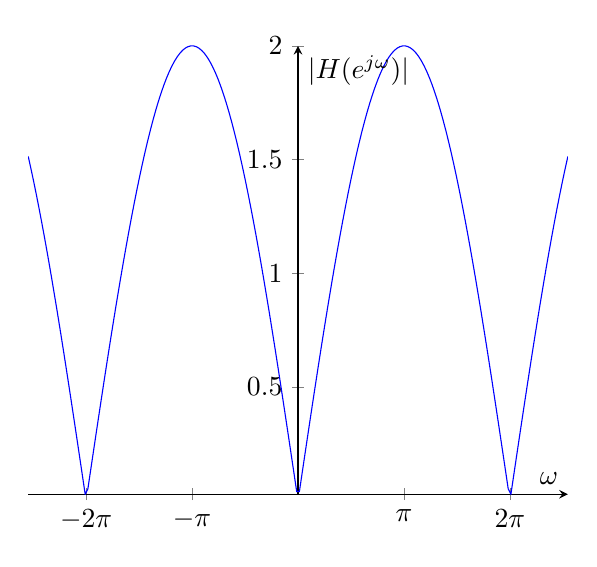
\begin{tikzpicture}
        \begin{axis}[
            xlabel=\(\omega\), ylabel={\(|H(e^{j \omega})|\)},
            axis lines=middle,
            xtick={-6.28318, -3.14159, 3.14159, 6.28318},
            xticklabels={\(-2\pi\), \(-\pi\), \(\pi\), \(2\pi\)}
        ]
        \addplot[
            color=blue,
            domain=-8:8,
            samples=200
        ]{2*abs(sin(deg(x/2)))};
        \end{axis}
    \end{tikzpicture}
    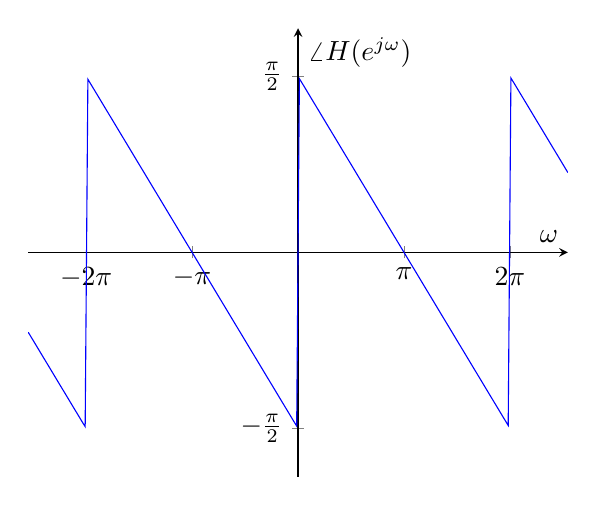
\begin{tikzpicture}
        \begin{axis}[
            xlabel=\(\omega\), ylabel={\(\angle H(e^{j \omega})\)},
            axis lines=middle,
            xtick={-6.28318, -3.14159, 3.14159, 6.28318},
            xticklabels={\(-2\pi\), \(-\pi\), \(\pi\), \(2\pi\)},
            ytick={-1.5708, 1.5708},
            yticklabels={\(-\frac{\pi}{2}\), \(\frac{\pi}{2}\)},
            ymin=-2, ymax=2
        ]
        \addplot[
            color=blue,
            domain=-8:8,
            samples=200
        ]{rad(atan2(sin(deg(x)), 1-cos(deg(x))))};
        \end{axis}
    \end{tikzpicture}
\end{center}
This seems to be consistent with the reasoning for part 3, when accounting for phase wrapping.

\end{document}
